\documentclass{standalone}

%\newif\iflabel

%\labeltrue

%\iflabel
%\newcommand{\lab}[1]{\tiny \textcolor{white}{\!#1\!}}
%\else
\newcommand{\lab}[1]{}
%\fi

\usepackage{amssymb,amsfonts,amsmath}
\usepackage{tikz,tkz-euclide}
\usetikzlibrary{arrows,calc,patterns}
\usepackage{pgfplots}

\begin{document}
  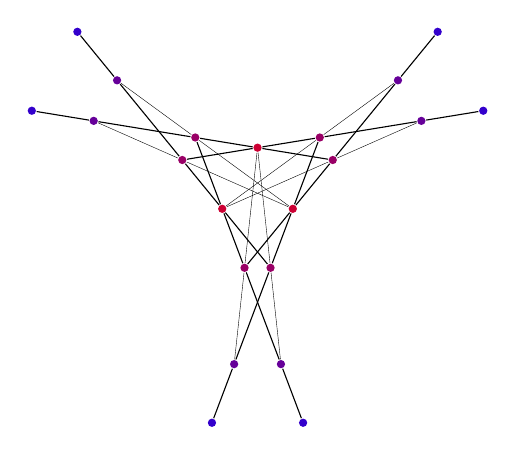
\begin{tikzpicture}[dot/.style={inner sep=1pt, circle, minimum size=1.5mm, thick, scale=0.7}]
    \begin{axis}[
      unit vector ratio=1 1 1,
      xmin=-6,xmax=6,
      ymin=-6.5,ymax=4.5,
      axis lines=none,
      xticklabel=\empty,
      yticklabel=\empty ]


\node[dot, fill=blue!60!red] (1) at (axis cs:-3.44617464571732, 2.6528664791724785) {\lab{1}};
\node[dot, fill=blue!60!red] (2) at (axis cs:-0.5743624409528887, -4.310908028655276) {\lab{2}};
\node[dot, fill=blue!60!red] (3) at (axis cs:4.020537086670208, 1.6580415494827958) {\lab{3}};
\node[dot, fill=blue!60!red] (4) at (axis cs:-4.020537086670213, 1.6580415494828025) {\lab{4}};
\node[dot, fill=blue!60!red] (5) at (axis cs:0.5743624409528854, -4.310908028655283) {\lab{5}};
\node[dot, fill=blue!60!red] (6) at (axis cs:3.4461746457173277, 2.652866479172479) {\lab{6}};
\node[dot, fill=blue!40!red] (7) at (axis cs:1.8462633705058416, 0.6978219618694791) {\lab{7}};
\node[dot, fill=blue!40!red] (8) at (axis cs:-1.5274632315505863, 1.25) {\lab{8}};
\node[dot, fill=blue!40!red] (9) at (axis cs:-0.3188001389552556, -1.9478219618694799) {\lab{9}};
\node[dot, fill=blue!20!red] (10) at (axis cs:0.8660254037844384, -0.5000000000000003) {\lab{10}};
\node[dot, fill=blue!20!red] (11) at (axis cs:0, 1) {\lab{11}};
\node[dot, fill=blue!20!red] (12) at (axis cs:-0.8660254037844387, -0.4999999999999998) {\lab{12}};
\node[dot, fill=blue!80!red] (13) at (axis cs:5.538790111517523, 1.906534114391559) {\lab{13}};
\node[dot, fill=blue!80!red] (14) at (axis cs:-4.420502032003517, 3.84346588560844) {\lab{14}};
\node[dot, fill=blue!80!red] (15) at (axis cs:-1.118288079514007, -5.7499999999999964) {\lab{15}};
\node[dot, fill=blue!40!red] (16) at (axis cs:1.5274632315505863, 1.25) {\lab{16}};
\node[dot, fill=blue!40!red] (17) at (axis cs:-1.846263370505841, 0.6978219618694803) {\lab{17}};
\node[dot, fill=blue!40!red] (18) at (axis cs:0.3188001389552543, -1.9478219618694796) {\lab{18}};
\node[dot, fill=blue!80!red] (19) at (axis cs:-5.538790111517525, 1.9065341143915626) {\lab{19}};
\node[dot, fill=blue!80!red] (20) at (axis cs:1.1182880795140007, -5.750000000000002) {\lab{20}};
\node[dot, fill=blue!80!red] (21) at (axis cs:4.420502032003524, 3.8434658856084365) {\lab{21}};

  \draw[line width=0.05mm] (1) -- (8) -- (10);
  \draw[line width=0.05mm] (11) -- (9) -- (2);
  \draw[line width=0.05mm] (3) -- (7) -- (12);
  \draw[line width=0.05mm] (10) -- (17) -- (4);
  \draw[line width=0.05mm] (11) -- (18) -- (5);
  \draw[line width=0.05mm] (6) -- (16) -- (12);
  \draw (14) -- (1) -- (17) -- (12) -- (18);
  \draw (16) -- (10) -- (18) -- (2) -- (15);
  \draw (13) -- (3) -- (16) -- (11) -- (17);
  \draw (7) -- (11) -- (8) -- (4) -- (19);
  \draw (8) -- (12) --  (9) --  (5) --  (20);
  \draw (21) -- (6) -- (7) -- (10) -- (9);

    \end{axis}
  \end{tikzpicture}
\end{document}
